\documentclass[11pt,a4paper]{article}
\usepackage[margin=1in]{geometry}
\usepackage[T1]{fontenc}
\usepackage{lmodern}
\usepackage{amsmath}
\usepackage{graphicx}
\usepackage{booktabs}
\usepackage[hidelinks]{hyperref}
\usepackage{enumitem}
\usepackage[font=small,labelfont=bf]{caption}
\setlist{itemsep=1pt,topsep=3pt}

\title{\Large\bfseries Does Practising Collisions Help?\\ Robustness and Reliability of Neuroevolved Driving Agents\\ Trained With and Without Simulated Collisions}
\author{Madhur Devidas Rathod\\ \small Independent researcher \quad·\quad \href{mailto:madhur.rathod1@adypu.edu.in}{madhur.rathod1@adypu.edu.in}}
\date{\small Technical report, November 2026}

\begin{document}
\maketitle

\begin{abstract}
\noindent
Agents trained in simulation are usually evaluated under the conditions they were trained in, yet the moment they matter most is when something unexpected happens. We study one simple form of this question in a small driving task: does exposing a neuroevolved driving agent to simulated collisions during training make it more robust to collisions it has never seen? We train a 132-weight neural-network driver with a genetic algorithm under two conditions that differ only in whether 3 of its 18 training drives include sideways shoves, and repeat each condition with 15 random seeds (30 networks). A standard held-out test proved too easy (most networks passed every drive), so we added a stress test that applies shoves up to 4$\times$ stronger. Typical robustness was similar in both conditions (median score 181 vs.\ 184 of 252), but collision training removed the bad outcomes: all 15 collision-trained runs solved training and the weakest scored 160, while calm training produced one run that never learned to drive and several fragile networks (scores 0, 99, 105, 128). Mean robustness was 30 points higher with collision training (95\% bootstrap CI 5.6--59.3; permutation $p=0.034$), but the effect is concentrated in the worst runs and is not significant under a rank test (Mann--Whitney $p=0.10$). We read this as evidence that cheap perturbations during training act mainly as insurance against unreliable evolutionary runs, and we release all code and results.
\end{abstract}

\section{Introduction}
Neuroevolution, training neural networks with evolutionary algorithms instead of gradient descent, is a simple and surprisingly competitive way to learn control policies \cite{stanley2002neat,floreano2008,such2017deep,salimans2017es}. A recurring problem with any learned controller is that it is optimised for the situations it practised on. In robotics, a common answer is to perturb or randomise the training conditions so the policy cannot rely on them being exactly right \cite{tobin2017dr,pinto2017rarl}.

This report asks a small, concrete version of that question. A browser racing game contains an AI car driven by a neural network that was trained by a genetic algorithm. Its training drives include a few in which the car is shoved sideways and spun, as if hit by another car. \textbf{Does that collision practice actually make the driver more robust to collisions, or would an agent trained on calm drives cope just as well?}

Because a single evolutionary run can be lucky or unlucky, we follow the advice to compare many independent runs and report their spread, not just their best result \cite{henderson2018matters,agarwal2021precipice}. Our contributions are:
\begin{itemize}
  \item A controlled comparison of two training conditions that differ only in the presence of shoves, with 15 seeded, reproducible runs per condition.
  \item A stress test that measures how each network degrades as collisions get stronger, introduced after the standard test showed a ceiling effect.
  \item The finding that collision practice mainly improves \emph{reliability} (no failed or fragile runs) rather than the robustness of a typical run.
\end{itemize}

\section{Setup}
\paragraph{Task.} A car drives a closed loop 577\,m long and 14\,m wide, seen from above, with three 12\,cm speed bumps. The physics run at a fixed 120\,Hz step and are fully deterministic: the car has tyre grip limits, can skid, and is damaged by taking a bump faster than its safe speed (40\,km/h for the car used here; top speed 115\,km/h). The simulation runs headless in Node.js, without graphics.

\paragraph{Network.} The driver is a fully connected network with 10 inputs, one hidden layer of 10 $\tanh$ units and 2 $\tanh$ outputs (steering and throttle/brake), 132 weights including biases. Its inputs are the distance to the road edge along 7 rays from $-90^\circ$ to $+90^\circ$ (range 40\,m), the car's speed, its sideways slip, and the distance to the next speed bump (range 60\,m), all scaled to roughly $[0,1]$. The network cannot see other cars.

\paragraph{Evolution.} A population of 80 networks starts from random Gaussian weights. Each generation, every network drives all training drives and receives a fitness: the mean over drives of
\begin{equation}
  F = \text{distance driven (m)} + 20\,(75 - t_{\text{finish}})\,[\text{finished}] - 30 \cdot \text{damage}(\%).
\end{equation}
A drive ends when the car's centre comes within 1.5\,m of the asphalt edge (relaxed to the outer curb for 2.5\,s after a shove), when it falls behind 2\,m/s of average progress, after 75\,s, or when it completes 1.25 laps; it counts as finished only with at most 3\% damage. The 8 best networks pass unchanged to the next generation (elitism); the other 72 are produced by tournament selection (best of 3), uniform crossover with probability 0.5, and Gaussian mutation (each weight with probability 0.15, $\sigma=0.4$). Training stops 25 generations after the best network first finishes every training drive, or after 300 generations.

\section{Experiment}
\paragraph{Conditions.} Both conditions use the same 18 training drives: 12 standing starts spread round the loop in different lanes, 3 starts just before the speed bumps, and 3 further drives. In the \textbf{shoves} condition those last 3 drives each contain 2--3 shoves (a sideways velocity change of 4--5\,m/s with a spin of 1--1.5\,rad/s, and in one case a backward push of 15\,m/s). In the \textbf{calm} condition the same 3 drives start in the same places but contain no shoves. Keeping the number and placement of drives identical means the conditions differ in one thing only.

\paragraph{Seeds.} Every run starts from random networks (no warm start) with a seeded random-number generator, so each run can be repeated exactly; we verified that two runs with the same seed produce identical networks. We first ran 5 seeds per condition as a pilot. Because the pilot was inconclusive, we extended both conditions to 15 seeds. We report all 30 runs, including one that failed to train.

\paragraph{Held-out test.} The final network of each run drives 108 drives it never trained on: 12 start points placed halfway between the training starts $\times$ 3 lanes, each run once without shoves, once with two shoves at times and strengths not used in training, and once with those shoves 1.4$\times$ stronger. A drive passes if the car completes 3 laps with its wheels on the asphalt (except for 2.5\,s after a shove) and at most 3\% damage. This test was fixed before any results were seen.

\paragraph{Stress test.} The held-out test showed a ceiling effect (Section~\ref{sec:results}), so we added a stress test after seeing those results: the 36 shoved drives are repeated with the shove strength multiplied by 1, 1.5, 2, 2.5, 3, 3.5 and 4. A network's \textbf{robustness score} is the number of passed drives summed over the 7 levels (maximum 252). Because the stress test and score were defined after the first results, the statistical tests below should be read as exploratory.

\paragraph{Statistics.} We compare robustness scores between conditions with a two-sided permutation test on the difference in means (100{,}000 permutations), a 95\% bootstrap confidence interval for that difference, a Mann--Whitney $U$ test (which uses ranks and so is less sensitive to extreme runs), and Levene's test for a difference in spread.

\section{Results}\label{sec:results}
\paragraph{Training.} All 15 collision-trained runs solved every training drive (median generation of first success 16, range 9--71). Calm training solved 14 of 15 (median 18.5, range 8--112); calm seed 15 never solved the training drives within 300 generations and failed every test drive. A run took 6--16 minutes on one CPU core.

\paragraph{Held-out test: a ceiling effect.} Most networks of both conditions passed all or nearly all held-out drives (Table~\ref{tab:heldout}). The test therefore could not separate the conditions, except through the calm networks that failed or nearly failed.

\begin{table}[h]
\centering\small
\caption{Held-out test: drives passed out of 36 per network, over 15 networks per condition.}
\label{tab:heldout}
\begin{tabular}{lcccccc}
\toprule
 & \multicolumn{2}{c}{Calm drives} & \multicolumn{2}{c}{Shoved drives} & \multicolumn{2}{c}{Hard shoves (1.4$\times$)} \\
Training & mean & min & mean & min & mean & min \\
\midrule
Calm   & 33.4 & 0  & 32.9 & 0  & 30.9 & 0 \\
Shoves & 35.8 & 34 & 35.5 & 33 & 35.0 & 31 \\
\bottomrule
\end{tabular}
\end{table}

\paragraph{Stress test.} Performance falls as the shoves get stronger in both conditions (Figure~\ref{fig:robust}). The median collision-trained network is at or above the median calm network at every strength (by up to 5 of 36 drives), but the clearest difference is in the spread: the calm networks fan out widely, while the collision-trained networks stay close together.

\begin{figure}[h]
\centering
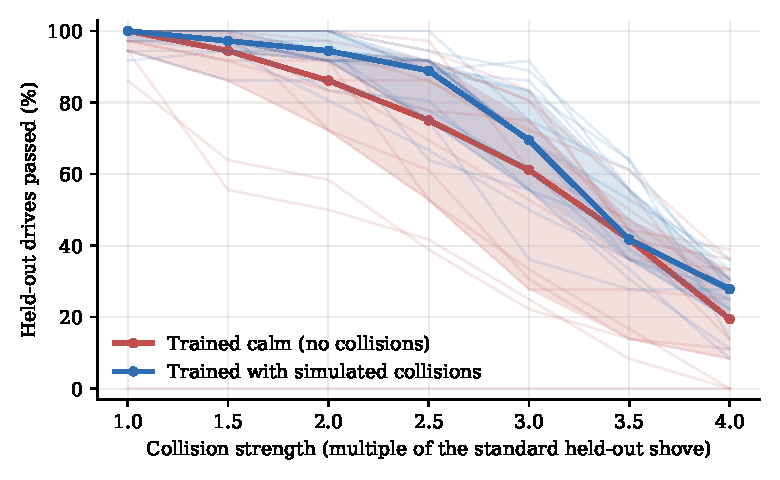
\includegraphics[width=0.82\linewidth]{fig_robustness.pdf}
\caption{Share of the 36 shoved held-out drives passed as shove strength increases. Bold lines: median of 15 networks per condition; bands: interquartile range; thin lines: individual networks. The calm network that never learned to drive lies at 0\%.}
\label{fig:robust}
\end{figure}

\begin{table}[h]
\centering\small
\caption{Robustness score per network (drives passed over the 7 stress levels, maximum 252).}
\label{tab:score}
\begin{tabular}{lccccc}
\toprule
Training & mean & median & s.d. & worst & networks \\
\midrule
Calm   & 153.7 & 181 & 53.7 & 0 (99 if the failed run is excluded) & 15 \\
Shoves & 183.7 & 184 & 16.7 & 160 & 15 \\
\bottomrule
\end{tabular}
\end{table}

Table~\ref{tab:score} summarises the robustness scores. The calm scores were 0, 99, 105, 128, 140, 151, 170, 181, 183, 186, 186, 192, 192, 196, 196; the collision-trained scores ranged from 160 to 207. With all 30 runs, collision training raised the mean score by 30.0 points (95\% CI 5.6 to 59.3; permutation $p=0.034$; Cohen's $d=0.75$). The rank-based Mann--Whitney test did not reach significance ($p=0.097$), and neither did Levene's test for spread ($p=0.097$). Excluding the calm run that never learned to drive, the difference was 19.0 points (95\% CI 0.9 to 38.7; permutation $p=0.064$; Mann--Whitney $p=0.16$). In the 5-seed pilot alone it was 29.0 points (95\% CI $-2.2$ to 65.8; $p=0.18$), which is why we extended the study.

\paragraph{How the drives failed.} Among networks that solved training, most failures in both conditions were the car leaving the road (890 failed drives for calm networks, 776 for collision-trained). The clearest qualitative difference was in drives that ended because the car stopped making progress, typically after being spun round and stalling or driving the wrong way: 155 for calm networks against 45 for collision-trained ones, about 3.4 times as many. Damage failures (taking a bump too fast) were slightly more common in collision-trained networks (194 vs.\ 154).

\section{Discussion}
The typical network learns to recover from shoves whether or not it practised them: the medians of the two conditions are close at almost every strength. What collision practice changes is the lower tail. Without shoves in training, some evolutionary runs settle on driving strategies that work on calm roads but fall apart after a hard knock, most visibly by getting spun round and failing to set off again, and one run never learned to drive at all. With shoves in training, none of the 15 runs did either.

A plausible reading is that the shoved drives put the car into states (pointing sideways, near the edge, at low speed) that calm drives rarely visit, so the fitness function penalises strategies that cannot recover from them. Calm training only rewards recovery indirectly, so whether a run happens to learn it depends on the seed. This fits the broader idea behind training-time perturbation and domain randomisation \cite{tobin2017dr,pinto2017rarl}: the main benefit may be to make good behaviour less dependent on luck. For a practitioner who will train one network and use it, that is the property that matters. Here it came at no measurable cost in training time.

\section{Limitations}
\begin{itemize}
  \item \textbf{Small scale.} One track, one car, one small network, and 15 runs per condition. The evidence for a difference in mean robustness is moderate and depends on the analysis; the rank-based test is not significant.
  \item \textbf{Exploratory analysis.} The stress test and robustness score were defined after the held-out test showed a ceiling effect, and the number of seeds was increased after a pilot. Both decisions are reported, but they make the $p$-values exploratory rather than confirmatory.
  \item \textbf{Simplified collisions.} A ``shove'' is an instantaneous change of velocity and spin, not a physical collision with another car, and the network cannot see other cars.
  \item \textbf{One perturbation recipe.} We tested one amount of collision practice (3 of 18 drives). How much practice helps, and whether other perturbations help in the same way, is untested.
\end{itemize}

\section{Conclusion}
In 30 seeded neuroevolution runs, practising simulated collisions did not make the typical driving agent much more robust, but it made training reliable: every collision-trained run produced a competent, collision-tolerant driver, while calm training occasionally produced fragile or failed ones. Future work could vary the amount and strength of collision practice, give the network sensors for other cars and train it in traffic, and test whether the reliability effect holds for larger networks and other tasks.

\paragraph{Reproducibility.} The simulator, the experiment and stress-test scripts, the analysis script, all 30 trained networks and their per-drive results are available at \url{https://github.com/madhurrathod/neuroevolution-collision-robustness}. One run: \texttt{node experiment.mjs --condition shoves --seed 1}; stress test: \texttt{node stress.mjs results/shoves\_seed1.json}.

\paragraph{Use of AI tools.} The author used Claude (Anthropic), an AI assistant, throughout this work: to write the game and simulation code under the author's direction, to write the experiment, stress-test and analysis scripts, and to draft this report. The author ran all experiments on his own computer, checked the reported numbers against the result files, and takes full responsibility for the content of this report.

\begin{thebibliography}{9}\small
\bibitem{stanley2002neat} K.~O. Stanley and R.~Miikkulainen. Evolving neural networks through augmenting topologies. \emph{Evolutionary Computation}, 10(2):99--127, 2002.
\bibitem{floreano2008} D.~Floreano, P.~D\"urr, and C.~Mattiussi. Neuroevolution: from architectures to learning. \emph{Evolutionary Intelligence}, 1(1):47--62, 2008.
\bibitem{such2017deep} F.~P. Such, V.~Madhavan, E.~Conti, J.~Lehman, K.~O. Stanley, and J.~Clune. Deep neuroevolution: Genetic algorithms are a competitive alternative for training deep neural networks for reinforcement learning. arXiv:1712.06567, 2017.
\bibitem{salimans2017es} T.~Salimans, J.~Ho, X.~Chen, S.~Sidor, and I.~Sutskever. Evolution strategies as a scalable alternative to reinforcement learning. arXiv:1703.03864, 2017.
\bibitem{tobin2017dr} J.~Tobin, R.~Fong, A.~Ray, J.~Schneider, W.~Zaremba, and P.~Abbeel. Domain randomization for transferring deep neural networks from simulation to the real world. In \emph{IROS}, 2017. arXiv:1703.06907.
\bibitem{pinto2017rarl} L.~Pinto, J.~Davidson, R.~Sukthankar, and A.~Gupta. Robust adversarial reinforcement learning. In \emph{ICML}, 2017. arXiv:1703.02702.
\bibitem{henderson2018matters} P.~Henderson, R.~Islam, P.~Bachman, J.~Pineau, D.~Precup, and D.~Meger. Deep reinforcement learning that matters. In \emph{AAAI}, 2018. arXiv:1709.06560.
\bibitem{agarwal2021precipice} R.~Agarwal, M.~Schwarzer, P.~S. Castro, A.~Courville, and M.~G. Bellemare. Deep reinforcement learning at the edge of the statistical precipice. In \emph{NeurIPS}, 2021. arXiv:2108.13264.
\end{thebibliography}

\end{document}
